\documentclass[11pt,letterpaper]{article}
\usepackage[margin=0.68in,headheight=15pt,headsep=17pt,footskip=25pt]{geometry}
\usepackage[T1]{fontenc}
\usepackage{lmodern,microtype}
\DisableLigatures{encoding=*,family=lmtt}
\usepackage[table]{xcolor}
\usepackage{tabularx,booktabs,array,enumitem}
\usepackage{tikz}
\usetikzlibrary{arrows.meta,positioning}
\usepackage{listings}
\usepackage{fancyhdr,lastpage}
\usepackage{hyperref}
\definecolor{ink}{HTML}{233240}
\definecolor{accent}{HTML}{255F7D}
\definecolor{soft}{HTML}{F1F5F7}
\definecolor{muted}{HTML}{586975}
\hypersetup{colorlinks=true,urlcolor=accent,linkcolor=accent,
 pdftitle={ContextShadow: Design Proposal},pdfsubject={Independent context histories over Git}}
\pagestyle{fancy}
\fancyhf{}
\fancyhead[L]{\small\textcolor{ink}{ContextShadow}}
\fancyhead[R]{\small\textcolor{muted}{Design proposal / v0.1}}
\fancyfoot[L]{\small\textcolor{muted}{15 October 2026}}
\fancyfoot[R]{\small\thepage\ / \pageref*{LastPage}}
\renewcommand{\headrulewidth}{0.3pt}
\setlength{\parindent}{0pt}
\setlength{\parskip}{6pt}
\setlength{\tabcolsep}{7pt}
\renewcommand{\arraystretch}{1.16}
\setlist[itemize]{leftmargin=16pt,itemsep=2pt,topsep=3pt,parsep=0pt}
\setlist[enumerate]{leftmargin=18pt,itemsep=2pt,topsep=3pt,parsep=0pt}
\newcolumntype{Y}{>{\raggedright\arraybackslash}X}
\newcommand{\sect}[1]{\vspace{5pt}{\large\bfseries\textcolor{ink}{#1}}\par\vspace{1pt}}
\newcommand{\subsect}[1]{\vspace{3pt}{\bfseries\textcolor{ink}{#1}}\par}
\newcommand{\code}[1]{{\small\texttt{#1}}}
\newcommand{\note}[1]{\begingroup\setlength{\fboxsep}{9pt}\colorbox{soft}{\parbox{\dimexpr\linewidth-18pt\relax}{#1}}\endgroup\par}
\lstset{basicstyle=\ttfamily\footnotesize,columns=fullflexible,keepspaces=true,
 breaklines=true,showstringspaces=false,backgroundcolor=\color{soft},
 frame=none,xleftmargin=7pt,xrightmargin=7pt,aboveskip=6pt,belowskip=6pt}
\begin{document}
{\LARGE\bfseries\textcolor{ink}{ContextShadow}}\par
{\large Independent context histories over Git}\par
\textcolor{muted}{A tool contract for coding harnesses. Proposed behavior; no commands are implemented by this document.}

\sect{1. Purpose and boundary}
ContextShadow is a Git-backed extension, exposed as \code{git cs}, for versioning
captured context. Callers can checkpoint, traverse, branch, merge, and replay
context independently of source code. Each CS checkpoint identifies a complete
active context. A code commit may reference the exact CS checkpoint associated
with its creation.

The extension stores and transforms data. The caller chooses what to capture,
when to checkpoint, which context to load, and whether to obtain a summary from
an LLM. Captured context means supplied data, not a model's hidden internal state.

\subsect{Independent histories are the default}
Code and context have separate commit graphs and refs. There is no requirement
that their branches, merges, or update frequency correspond. A CS operation
does not move a code ref or modify code files. A code operation does not move
a CS ref unless an explicitly combined command requests it.

\begin{center}
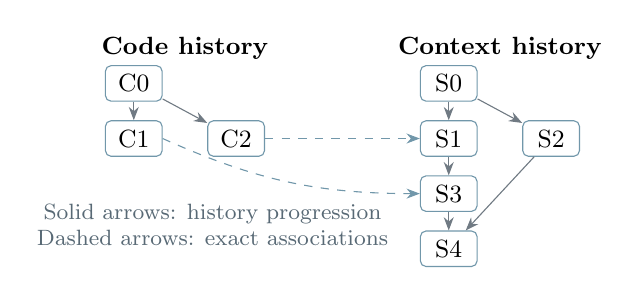
\begin{tikzpicture}[x=1cm,y=1cm,>=Stealth,
 revision/.style={draw=accent!65,fill=white,rounded corners=2pt,
 minimum width=0.72cm,minimum height=0.42cm,font=\small},
 history/.style={->,draw=ink!65,thin},
 association/.style={->,draw=accent!65,dashed,thin}]
 \node[font=\small\bfseries] at (0.65,0.45) {Code history};
 \node[font=\small\bfseries] at (4.65,0.45) {Context history};
 \node[revision] (c0) at (0,0) {C0};
 \node[revision] (c1) at (0,-0.70) {C1};
 \node[revision] (c2) at (1.3,-0.70) {C2};
 \node[revision] (s0) at (4,0) {S0};
 \node[revision] (s1) at (4,-0.70) {S1};
 \node[revision] (s2) at (5.3,-0.70) {S2};
 \node[revision] (s3) at (4,-1.40) {S3};
 \node[revision] (s4) at (4,-2.10) {S4};
 \draw[history] (c0)--(c1);
 \draw[history] (c0)--(c2);
 \draw[history] (s0)--(s1);
 \draw[history] (s0)--(s2);
 \draw[history] (s1)--(s3);
 \draw[history] (s3)--(s4);
 \draw[history] (s2)--(s4);
 \draw[association] (c1.east) to[bend right=12] (s3.west);
 \draw[association] (c2.east)--(s1.west);
 \node[font=\footnotesize,text=muted,align=center] at (1,-1.8)
 {Solid arrows: history progression\\Dashed arrows: exact associations};
\end{tikzpicture}
\end{center}

The diagram has a context merge without a code merge. Two code branches refer
to checkpoints on one context path. Traversing either graph is independent;
association queries provide the cross-history view.

\subsect{Why accept the extra graph?}
Investigation can advance without code changes, and one context can support
several implementations. Code and context can be integrated at different times.
The cost is an ambiguous paired restore: a context checkpoint may have zero,
one, or several associated code commits. Context-only checkout is guaranteed;
reconstructing a complete development environment is a separate caller concern.

\note{\textbf{Core promise:} preserve exact context states and their history,
with explicit associations to code. An association records provenance supplied
by a caller; it does not certify correctness, causal completeness, or that an
agent actually consumed every stored item.}

\newpage
\sect{2. Checkpoints are states; chunks are content}
A CS checkpoint is an ordinary Git commit whose tree contains a manifest and
immutable chunks. The manifest resolves the complete active context without
replaying application state through its ancestors. Git parents record history.

\rowcolors{2}{soft}{white}
\begin{tabularx}{\linewidth}{p{1.45in}Y}
\toprule
\textbf{Identity} & \textbf{Meaning}\\
\midrule
Checkpoint ID & Full Git object ID. A change to contents, parents, or commit metadata creates a new ID.\\
Chunk ID & Stable UUID assigned when content is first captured. The same UUID must always identify the same chunk bytes.\\
Branch name & Moving ref under \code{refs/cs/heads/}. It identifies a path, not an immutable revision.\\
Session ID & Optional caller metadata. It is not required for checkpoint identity or ancestry.\\
\bottomrule
\end{tabularx}
\rowcolors{2}{}{}

\subsect{Minimal format: \code{cs/1}}
The tree contains \code{context.json} and \code{chunks/<uuid>.json}. Every active
chunk must be present as a normal Git-tree entry; IDs embedded in JSON alone
are not native Git reachability links.
\begin{lstlisting}
// context.json -- illustrative UUIDs abbreviated
{ "schema": "cs/1", "active": ["m1", "m2", "a1"] }

// chunks/a1.json
{ "id": "a1", "kind": "message", "body": "Investigate SQLite." }
\end{lstlisting}
An \code{active} list contains unique IDs in presentation order. Envelopes use
UTF-8 JSON with deterministic serialization. Import preserves the declared
chunk identity and compares canonical stored bytes. Different IDs with identical
text remain distinct. Reusing one ID with different bytes is an identity conflict.

Messages, tool exchanges, summaries, and opaque records can be chunks. The
caller chooses atomic boundaries; the extension never splits a chunk during
merge. Editing creates a new chunk ID. Omitting an old chunk changes the active
view; the old bytes remain in historical checkpoints.

\subsect{Summaries change the active view}
A summary is a new chunk containing its text and the full CS checkpoint IDs
it summarizes. A caller may replace many active chunks with that summary in
a new checkpoint. The sources remain accessible through history or declared
dependency refs. A summary is supplied content, not a tool-generated judgment.

\subsect{What is versioned?}
\begin{itemize}
\item The active ordered view and each referenced chunk's exact contents.
\item Commit ancestry, author/committer metadata, and declared summary sources.
\item Caller-provided records, which the core treats as data unless a driver interprets them.
\end{itemize}
The extension does not infer agreement, task completion, validity of tool
exchanges, or token-budget suitability. Optional format drivers can validate
more. Their identifiers and versions must be recorded so peers can reproduce
the mechanical transformation or reject an unsupported format.

\note{\textbf{Storage choice:} a complete state assembled from reusable chunks.
This supports direct historical checkout while keeping message identity and
merge boundaries explicit. It avoids requiring a caller to reconstruct state
by interpreting every prior event.}

\newpage
\sect{3. Merge, replay, and concurrent writers}
\subsect{Default merge: ordered union}
For divergent \code{cs/1} histories, an omitted result selects ordered union
of the two tips' active lists. Common ancestry identifies the histories;
the union algorithm operates on their active content:
\begin{enumerate}
\item Combine active chunk IDs, including a shared ID once. Validate that every shared ID has identical bytes.
\item Preserve each source's order by adding precedence edges between adjacent IDs in its active list.
\item Topologically order the combined IDs. Break ties between unconstrained IDs by UUID byte order.
\item If the precedence constraints cycle, return an order conflict. Do not advance the destination ref.
\end{enumerate}
The result is deterministic for the same inputs and driver version. It preserves
each input order and keeps whole chunks intact. The chosen order between
independent additions is a mechanical convention, not a claim about chronology.

\rowcolors{2}{soft}{white}
\begin{tabularx}{\linewidth}{p{1.45in}Y}
\toprule
\textbf{Input/result} & \textbf{Active chunk sequence}\\
\midrule
Base & M1, M2\\
Branch A / branch B & M1, M2, A1 \quad / \quad M1, M2, B1\\
Union & M1, M2, A1, B1, assuming A1 sorts before B1\\
Supplied summary & S1, or any valid caller-supplied active view\\
\bottomrule
\end{tabularx}
\rowcolors{2}{}{}

Union retains any chunk active on either side. Removal on only one side does
not remove it from the result. It does not infer supersession or deduplicate
a summary against the messages it covers. Callers choose another driver or
supply a result when those rules are unsuitable.

\subsect{Supplied results and text drivers}
\code{git cs merge agent-b --result merged-context.json} imports and validates
a complete result, then creates a checkpoint with both source tips as parents.
The supplied file is a self-contained interchange payload containing its
manifest and required chunks. A human, script, or LLM may produce it.
An omitted result means union; an explicit zero-entry context means an empty
active view. A zero-byte or malformed payload is invalid.

Fast-forward merges may only advance a ref; \code{--no-ff} requests an explicit
merge checkpoint. Plain text formats can instead use Git's three-way text or
union drivers. Git's line-union driver does not preserve message boundaries
and warns that resulting line order may be unsuitable [3].

\subsect{Rebase and cherry-pick replay data}
The first implementation supports linear replay. Additions replay using the
defined chunk and order rules. Replacements, removals, and reorders require
their expected input state to match, or an explicit resolution. A summary
retains its original source scope; replay does not regenerate it. Histories
containing merge commits are rejected until merge-preserving replay is supported.
Revert creates a new state with inverse changes; it does not reverse tool effects.

\subsect{Concurrent updates}
Each caller supplies a CS ref and expected tip. Publish with a conditional
ref update [2]; if another writer advanced it, return \code{STALE\_TIP}.
Callers may share a branch or use separate branches. There is no
repository-global CS head. Moving a ref does not mutate any running agent's input.
Referenced originals remain pinned when branches are rebased or reset.

\newpage
\sect{4. Tool interface and code associations}
\subsect{Command contract}
All names and flags below are proposed. Every mutation supports \code{--json}
results. Branch-tip updates accept \code{--expect <checkpoint>}. Selection is
explicit or scoped by \code{--workspace <id>}, independently of Git's \code{HEAD}.

\rowcolors{2}{soft}{white}
\begingroup\small
\begin{tabularx}{\linewidth}{p{2.10in}Y}
\toprule
\textbf{Command family} & \textbf{Contract}\\
\midrule
\code{init; commit --input file} & Initialize CS state; validate and save a complete supplied context.\\
\code{branch; switch; reset} & Manage CS refs and caller-local selection. Save the previous tip under a recovery ref before reset.\\
\code{log; show; diff} & Traverse checkpoints, inspect complete payloads, and compare stored state.\\
\code{merge; merge-preview} & Compute union, use a configured driver, or accept a supplied result. Preview does not move a branch.\\
\code{rebase; cherry-pick; revert} & Apply recorded data transformations with explicit conflict handling.\\
\code{tag; label; reflog} & Name one checkpoint; group many checkpoints; inspect ref movement history.\\
\code{fetch; push; bundle} & Transfer selected CS refs and their declared dependency closure. Fetch does not integrate.\\
\code{links --code C} & Resolve the primary CS checkpoint associated with code commit C.\\
\code{links --context S} & Find associated code commits within specified code refs.\\
\code{fsck; pin; unpin} & Validate CS links and manage persistent dependency retention.\\
\bottomrule
\end{tabularx}
\endgroup
\rowcolors{2}{}{}

A label groups exact checkpoints: \code{label add ticket-42 S1 S2} and
\code{label resolve ticket-42}. Membership changes do not rewrite checkpoints
or implicitly label ancestors. A Git-style tag has one target.

\subsect{A code commit points to one exact CS checkpoint}
The prototype stores a trailer [6]:
\begin{lstlisting}
Context-Shadow: <full-CS-checkpoint-object-id>
\end{lstlisting}
The link means that the caller associated this code commit with that captured
context. Code ancestry preserves parent associations; squashing can remove
that path. Complete contributor attribution across squashes is a future
extension, not an implied guarantee.

The combined \code{git cs commit-code --context S -- <git-commit-options>}
validates S, pins its dependencies, and creates the code commit with the trailer.
It must validate the final link before publishing the commit. Failure may leave
an unused pin, but must not publish an unretained association. A post-commit
hook alone is too late to embed a link without changing the code commit ID.

The pointer is code-to-context only; reverse lookup scans selected code history
with a rebuildable cache. Neither history silently retargets existing links.
Ordinary Git and imported commits may be unlinked. Enforcement covers the
integrated commit path or separately configured repository checks.

\subsect{Historical branching}
\code{git cs switch -c retry S} selects a new CS branch at S. Reset moves an
existing branch and keeps a recovery ref. Both expose the recorded context at
that point; neither restores code, external resources, or unrecorded data.
Staging and editable context workspaces are optional later features.

For a cut inside a checkpoint, \code{branch retry S --through M} creates a
derived checkpoint with the active prefix through chunk M and parent S.
It is marked as a derived view, not an exact historical execution state.
Exact historical branching requires a checkpoint recorded at that boundary.
The caller validates that a selected boundary is resumable.

\newpage
\sect{5. Retention, transfer, and delivery}
\subsect{Refs and dependency closure}
CS objects use the existing Git object database. Heads, remote-tracking refs,
tags, labels, pins, and recovery refs live under \code{refs/cs/}. Git ancestry
and tree edges keep normal content reachable [1,4]. Trailers and checkpoint
IDs written in JSON do not create native reachability edges.

The extension pins exact CS checkpoints referenced by code and declared
summary dependencies. Transfer includes selected heads plus the recursively
required CS dependencies and pins, even when a rebase made an original
checkpoint unreachable from the new tip. Ref deletion or pruning must not
silently release an outstanding dependency. Git GC and packing remain
repository-wide; CS manages the retention roots.

\code{git cs push} uses explicit refspecs and must report unsupported custom
refs or missing dependencies. Ordinary \code{git push --all} is insufficient
because it selects \code{refs/heads/} [5]. Paired publication can send the code
ref and required CS pins in one atomic push when the endpoint supports it.
Otherwise publish CS dependencies first, then code, and report partial failure.
This ordering protects CS-aware transfers; ordinary Git pushes can still
deliver code whose context is unavailable.

Custom refs provide organization, not access control. Context export is
explicit because code and conversations can have different sharing audiences.
Generic Git commands such as \code{log --all} may include CS refs.

\subsect{First-build acceptance criteria}
\begin{enumerate}
\item Context commits, branches, and merges leave code refs and code files unchanged.
\item Two callers publishing from one expected tip cannot silently overwrite each other.
\item Union deduplicates shared IDs, preserves source order, retains distinct repeated text, and reports identity/order conflicts.
\item A supplied summary is active while both source histories remain recoverable.
\item A code-linked checkpoint remains readable after CS rebase, reset, branch deletion, and ordinary Git GC.
\item A fresh receiver can resolve every link in a CS-aware code transfer.
\item Interrupted operations leave either the old ref or a complete new checkpoint; retries detect stale tips and tolerate unused pins.
\end{enumerate}

\subsect{Scope and decisions still open}
The first build covers \code{cs/1}, checkpoint/traversal, branching/reset,
ordered union, supplied results, limited linear replay, labels, associations,
retention, and explicit exchange. It reuses Git plumbing rather than changing
Git core. Semantic resolution, agent execution, automatic capture, staging,
and paired environment restoration remain caller concerns or later features.

Before implementation, settle the external payload/driver versioning contract,
remote support for custom refs, and the policy for retiring pins when associated
code is intentionally removed. Native Git association support could later
replace trailer-and-pin conventions with built-in retention and transfer.

\subsect{Primary references}
{\footnotesize
[1] Git, commit objects: \url{https://git-scm.com/docs/git-commit-tree}\par
[2] Git, conditional ref updates: \url{https://git-scm.com/docs/git-update-ref}\par
[3] Git, merge drivers: \url{https://git-scm.com/docs/gitattributes}\par
[4] Git, garbage collection: \url{https://git-scm.com/docs/git-gc}\par
[5] Git, refspecs and atomic push: \url{https://git-scm.com/docs/git-push}\par
[6] Git, commit trailers: \url{https://git-scm.com/docs/git-interpret-trailers}
}
\end{document}
